\documentclass[sigconf]{acmart}

\usepackage{booktabs} % For formal tables


% Copyright
%\setcopyright{none}
%\setcopyright{acmcopyright}
%\setcopyright{acmlicensed}
\setcopyright{rightsretained}
%\setcopyright{usgov}
%\setcopyright{usgovmixed}
%\setcopyright{cagov}
%\setcopyright{cagovmixed}


% DOI
\acmDOI{}

% ISBN
\acmISBN{}

%Conference
\acmConference[PCSC2019]{Philippine Computing Science Congress}{March 2019}{City of Manila, Philippines}
\acmYear{2019}
\copyrightyear{2019}


\acmArticle{}
\acmPrice{}

% These commands are optional
%\acmBooktitle{Transactions of the ACM Woodstock conference}
\editor{}
\editor{}
\editor{}


\begin{document}
\title{ASSYSTX: Supporting Collaboration in Timetabling Systems}
%\titlenote{Produces the permission block, and
  %copyright information}
%\subtitle{Subtitle}
%\subtitlenote{The full version of the author's guide is available as
  %\texttt{acmart.pdf} document}


\author{Troy Michael Mirafuentes}
%\authornote{Dr.~Trovato insisted his name be first.}
%\orcid{1234-5678-9012}
\affiliation{%
  \institution{De La Salle University}
  %\streetaddress{P.O. Box 1212}
  \city{Manila, Philippines}
  %\state{Ohio}
  %\postcode{43017-6221}
}
\email{troy_mirafuentes@dlsu.edu.ph}

\author{Arvin Roi Ante}
%\authornote{Dr.~Trovato insisted his name be first.}
%\orcid{1234-5678-9012}
\affiliation{%
  \institution{De La Salle University}
  %\streetaddress{P.O. Box 1212}
  \city{Manila, Philippines}
  %\state{Ohio}
  %\postcode{43017-6221}
}
\email{arvin_ante@dlsu.edu.ph}

\author{Mark Gavin Sanchez}
%\authornote{Dr.~Trovato insisted his name be first.}
%\orcid{1234-5678-9012}
\affiliation{%
  \institution{De La Salle University}
  %\streetaddress{P.O. Box 1212}
  \city{Manila, Philippines}
  %\state{Ohio}
  %\postcode{43017-6221}
}
\email{mark_gavin_sanchez@dlsu.edu.ph}

\author{Jordan Aiko Deja}
%\authornote{Dr.~Trovato insisted his name be first.}
%\orcid{1234-5678-9012}
\affiliation{%
  \institution{De La Salle University}
  %\streetaddress{P.O. Box 1212}
  \city{Manila, Philippines}
  %\state{Ohio}
  %\postcode{43017-6221}
}
\email{jordan.deja@dlsu.edu.ph}

\author{Rafael Cabredo}
%\authornote{Dr.~Trovato insisted his name be first.}
%\orcid{1234-5678-9012}
\affiliation{%
  \institution{De La Salle University}
  %\streetaddress{P.O. Box 1212}
  \city{Manila, Philippines}
  %\state{Ohio}
  %\postcode{43017-6221}
}
\email{rafael.cabredo@dlsu.edu.ph}



% The default list of authors is too long for headers.
\renewcommand{\shortauthors}{T. Mirafuentes et al.}


\begin{abstract}
In a university setting, academic timetabling has been an open opportunity for developers and system designers. It is usually focused on generating schedules, managing conflicts, accommodating constraints and even allocating respective logistical needs. There are several off-the-shelf and customized systems that have been developed to accommodate the varying needs of different universities and organizations. The usage and the underlying human factors when using these systems is another consideration that we can tackle with these timetabling systems. In this paper, we attempt to discover, design, implement an academic timetabling system that considers human collaboration with other humans and with the computer itself. We iterated on developing a prototype for course scheduling, assigning of faculty and other pre-enrollment tasks. We observed stakeholders such as Department Chair, Academic Officers and other key personnel and inquired into their pains and struggles in academic timetabling. To help them in this process, we present ASSYSTX: An online platform that supports collaboration between key personnel involving in academic timetabling. We also identified key collaboration points towards providing affordances that cater to the needs of these personnel. 
\end{abstract}

%
% The code below should be generated by the tool at
% http://dl.acm.org/ccs.cfm
% Please copy and paste the code instead of the example below.
%
\begin{CCSXML}
<ccs2012>
 <concept>
  <concept_id>10010520.10010553.10010562</concept_id>
  <concept_desc>Computer systems organization~Embedded systems</concept_desc>
  <concept_significance>500</concept_significance>
 </concept>
 <concept>
  <concept_id>10010520.10010575.10010755</concept_id>
  <concept_desc>Computer systems organization~Redundancy</concept_desc>
  <concept_significance>300</concept_significance>
 </concept>
 <concept>
  <concept_id>10010520.10010553.10010554</concept_id>
  <concept_desc>Computer systems organization~Robotics</concept_desc>
  <concept_significance>100</concept_significance>
 </concept>
 <concept>
  <concept_id>10003033.10003083.10003095</concept_id>
  <concept_desc>Networks~Network reliability</concept_desc>
  <concept_significance>100</concept_significance>
 </concept>
</ccs2012>
\end{CCSXML}

\ccsdesc[500]{Computer systems organization~Embedded systems}
\ccsdesc[300]{Computer systems organization~Redundancy}
\ccsdesc{Computer systems organization~Robotics}
\ccsdesc[100]{Networks~Network reliability}


\keywords{ACM proceedings, \LaTeX, text tagging}


\maketitle

\section{Introduction}
Off-the-shelf Enrollment Systems are used by bigger universities in the Philippines while universities with smaller populations usually develop their own systems in-house. What is common with these systems is that their continued usage introduces a different set of problems for users coming from different backgrounds and technical proficiency. In general, most enrollment systems both off-the-shelf and developed in-house would be made to address common problems encountered in enrollment. Such issues would revolve around managing different block schedules, accommodating irregular students, allocating logistics such as classrooms, computer laboratories and field rooms, and assigning faculty. These tasks are usually pre-enrollment activities that are done in preparation for actual enrollment. Aside from this, there are other systems and modules that cater to the other stages of the Enrollment and Post-Enrollment Process. Regardless of the stage of enrollment concerned, human collaboration is an important aspect that is seldom considered when designing and developing key systems and features. As a matter of fact, even systems that have partial automation still require the human element especially when involved with key major decisions and time-pressed concerns. In Pre-enrollment activities alone, constant collaboration, communication and clarification is essentials towards the successful planning of enrollment in a given university. Users from varying levels and organization scope, who are involved in these stages are key decision makers who can implement changes in enrollment that will definitely affect the academic load of both faculty and students. 

In comparison, these systems are not entirely interactive and collaborative in nature. For key officials who are newly-placed into their posts, an additional learning curve prolongs the process. Most especially for off-the-shelf systems, they provided limited user feedback and do not give an avenue for collaboration between other key personnel involved. As such, these systems may generally hinder collaboration. To some organizations and universities, the collaborative aspects in the process of enrollment are relied from the usage of third-party tools such as Viber, Messenger, and other messaging platforms. These systems do not also give its current users insights on which portion of the work or process are being worked on by other key staff and personnel. As a result, either a feature may be locked to a certain user for a given moment or two users might be inputting conflicting information that could have been avoided if these users are aware of what they are both editing. The visual interface of these systems must be accompanied by design elements that guide all of its users towards understanding the process and the impacts of the changes they apply in the enrollment system. Our work makes an inquiry into the underlying design factors that affect the collaborative behaviors in enrollment and timetabling systems, specifically in the pre-enrollment process. We sought to understand the human factors involving key users and administrative personnel when operating an in-house designed software prototype with key collaborative features in supporting pre-enrollment. We did a formative study composed of interviews, observations, user tests with participants. We developed a prototype based on these findings which we iteratively tested as well. In this paper we: (1) Observe and understand how key personnel from a specific university, collaborate in pre-enrollment. We also (2) derive and formulate guidelines towards a collaborative online platform that these key personnel can use in planning their pre-enrollment deliverables such as course schedule, faculty schedule and block schedules. Additionally, we (3) discuss design implications for supporting these collaborative activities. Lastly, we (4) reflect on how we can design better enrollment systems that foster collaboration between key staff, and towards pushing it in different stages of the enrollment process. 

\section{Related Work}
\subsection{Academic Timetabling Systems}
There are several academic timetabling systems that been designed and developed to address various problems in an academic setting. One example is ASSYST. The Automated Scheduling System (ASSYST) \cite{Assyst} was developed to automate the course scheduling process. It had two modules for each user type: the College Academic Assistant (CAA) module and the Chair/Vice-Chair module. \cite{Assyst} generates an initial course schedule and improves it through Genetic Algorithms. ASSYST ver. 2 \cite{Assyst2} extended features of its predecessor to include faculty scheduling. The faculty schedules were also generated using Genetic Algorithms. A web-version of the system was developed after several years, named e-ASSYST \cite{eAssyst}. Unlike its predecessors, it used Tabu Search to create faculty schedules. The work in \cite{2013Nigeria} developed a timetabling system that utilizes Constraint-Satisfaction techniques to automate their timetabling process. The system was able to quickly generate lectures schedules that satisfied both soft and hard constraints given to it, and was successfully tested using the System Usability Scale method. \cite{UPM} is another web-based system that aimed to expedite creating course schedules for their departments following the specified constraints of the user. It boasted the ability to generate a timetabling schedule in the case an incomplete solution is found. \cite{Oprea2007} developed a timetabling system that operates through Multi-Agent Systems. The agents negotiate with one another in the case of conflicts, and help each other to form an optimal or sub-optimal timetabling schedule. The work in \cite{bulacanState}, meanwhile, addressed the decentralization of resources from university parent and satellite campuses. The system aids users assigned to create faculty and course schedules. The system was only designed to help evenly distribute the resources between university campuses through a centralized database system that stores university resources to guide its users in creating schedules. Another work in \cite{UniTime} is a commercial timetabling system that hosts multiple useful features such as: timetable creation, editing timetables, schedule conflict prevention, and room allocation. The same work in \cite{UniTime} also allows multiple ways to create the class schedules, offering centralized, distributed and hybrid approaches. It provides options for the users to customize the schedule, satisfying hard constraints imposed on the course scheduling process by departmental rules. The focus of \cite{Assyst, Assyst2, eAssyst, UPM, bulacanState, 2013Nigeria, Oprea2007, UniTime} have been towards automating the creation of course schedules and improving these generated schedules with optimization algorithms. However, most of these systems omit the human collaboration component that is essential in the enrollment process. For instance, \cite{Assyst} and \cite{Assyst2} have modules for each user type but it does not support collaboration between them. \cite{arrowSmith}, meanwhile, takes a more humanist approach and tackled the usability of academic timetabling systems. The course and faculty scheduling features remain but it does not rely on an optimization algorithm to create and improve these schedules. Their system focused, instead, on improving its user interface design by following a set of heuristics by \cite{Paz}. It was also verified iteratively through Keystroke-Level Modeling. Despite the change of focus, \cite{arrowSmith} also did not address human interaction and collaboration in their design and testing phases. Thus, collaboration within timetabling systems remains unexplored. This can put a damper towards deploying these systems to the involved personnel as collaboration is important when executing these processes. \cite{arrowSmith}, though, is in the right direction; its humanist approach lends itself to focusing on enhancing the user's interactions with the system. Nevertheless, collaboration is still lacking and therefore a factor to be considered.

% Discuss here the previous CCS systems such as ASSYST, ASSYST2, E-ASSYST, ArrowSmith etc. In the discussion, lets not mention DLSU. Lets mention how these systems were developed and what was their focus. Then conclude by saying, was collaboration a key issue. what key features of these systems worked and did not work and will work or used for assystx. 

\subsection{All-Purpose Collaboration Systems}
%\cite{Dix:2003:HI:1203012} talks about email as a good example of a CSCW system. Originally based on the conventional postal system, it allows communication between individuals who are at physically removed locations from each other. A user can create an email and send it to another person or a group of people. When a person receives the email, a notification would pop up to prompt the receiving person that a new email has just arrived. The email can be then viewed and the user may respond accordingly to its contents.

There are many systems outside the academic setting that have contributed to empowering collaboration within organizations. Google Docs \citep{googleDocs} is a proprietary online word processing application that allows users to write, edit, and collaborate on documents. The application boasts several collaborative features such as: document sharing, concurrent editing, online chat, and comments. It allows both asynchronous and synchronous collaboration between users in a single document. Asynchronous because user do not have to be working at the same time frame to write the document, and synchronous because it allows real time functions such as concurrent editing, and the chat features. Another example and from the similar suite, Google Sheets \cite{googleSheets} is a proprietary online spreadsheet application which allows users to create, edit, and collaborate on spreadsheets. The application also boasts the same collaborative features as \cite{googleDocs} and can also accommodate both asynchronous and synchronous collaboration. The two applications are for general use; it can be used for timetabling processes. However, timetabling requires a tailored application to fully capture its needs and intricacies, for example a feature for scheduling wherein the application can check for redundancies and errors. Thus, \cite{googleDocs} and \cite{googleSheets} cannot fully function as a timetabling application. The collaborative features of concurrent editing and messaging were used as inspiration for ASSYSTX's implementation especially on the communication aspects of collaboration. 

%The Google Calendar API is a tool that allows developers to add features that allow users to manage their respective calendar events\citep{googlecalendar}.  
%Slack is marketed as a collaboration hub and tool that allows users to manage their respective conversations \citep{slack}. The application makes use of channels that segregate a user's respective task, team, or anything that is relevant to the user. Collaborative channel functions include: message sending in the channel, a join-share function, a leave function, voice and video calls, screen-sharing, and file sharing. The application allows asynchronous collaboration as it does not require users to be online at the same time for its messaging, join-share, leave, and file sharing features. It also allows synchronous collaboration as users have to be online for its video call, screen-sharing, and also in its chat function.

%Trello is a project management collaboration tool that allows teams to keep track of progress in their projects \citep{trello}. The application makes use of a board that holds a collection of lists that represent project tasks and elements. Lists are filled with cards that represent a unit that is associated with the list. Collaborative features include: Adding of members to a Trello board, adding members to a card, card checklist and due dates, file sharing via attachments, comments, notifications, and real time board syncing. The application allows asynchronous collaboration as members do not have to be online to access any of the collaborative features. 

%Look at other related work outside dlsu put them here. same guide questions. 

\section{Methodology}
The methodology follows the Design Research approach as seen in the works of \cite{deja2018myosl, deja2018flow, chan2019applying}. It follows a human-centric methodology where user needs are extracted and transformed into features that are intended for the use-case concerned. These were derived from formative studies that were later processed into needfinding artefacts  that are used in the Prototype phases. This phase allows the development of a prototype that is iterated and tested by the intended users before actual deployment. More details are seen as described in Fig \ref{fig:pipelinediagram}. 
\begin{figure}[h]
   \centering
   \includegraphics[scale=0.18]{Diagrams/Methodology.png}
   \caption{The research methodology for ASSYSTX. The first phase (P1) dealt with understanding the stakeholders' needs and issues in the course scheduling and faculty load assignment processes. The second phase (P2) used the data to be gathered from the first to design and develop the existing system. The third phase (P3) involved repeatedly testing and validating the newly developed system with the stakeholders.}
    \label{fig:pipelinediagram}
\end{figure}
\subsection{Needfinding and User Research}
As a formative study, Stakeholder interviews and timetabling demonstration comprise the first phase, as it follows the Interaction Design process described in \cite{Dix:2003:HI:1203012}. The purpose is to gain a better understanding of the timetabling processes. The stakeholders involved are the Academic Programming Officer (APO), who is in charge of course scheduling, and the Department Chairs and Vice-Chairs, in charge of faculty scheduling. Informed consent was secured before conducting the interviews and demonstration. The interview was done to extract insights and understand the pains and struggles that hinder these key personnel from doing actual collaborative work. Below are some of the following questions that were asked during the interviews:
\begin{enumerate}
    \item How is course scheduling done? What are its difficulties?
    \item How is faculty load assignment done? What are its difficulties?
    \item How do you prioritize who should input data first when collaborating?
    \item How do you communicate with the other stakeholders, i.e. Chairs, Vice Chairs, APO, etc.?
    \item What are some features you would like to see in a timetabling application?
\end{enumerate}
Follow-up questions were also asked depending on the stakeholder's answers and roles. This is followed by a demonstration of the timetabling process is performed by the involved stakeholder. While in action, additional questions were also asked for clarity. Data collated -- interview answers and observations -- were processed into possible solutions to define the needs and issues of the stakeholders. These were then proposed to the stakeholders with the goal of garnering comments and suggestions. These were processed into artefacts such as Personas, affinity diagrams, empathy maps and scenario maps. This process was iterated until both stakeholders and researchers were satisfied with the insights and initial designs that will later on be used to develop the prototype. 

\subsection{Iterative Prototyping}
We designed an initial prototype that follows the seven principles summarizing the user-centered design process \cite{Norman:2002:DET:2187809}. We came up with different prototype mockups as possible solutions to present to the stakeholders. The stakeholders also explored the previous Arrowsmith system to provide suggestions for improvements in line with the prototypes. Once we had finalized and agreed upon the interface design, we proceeded to development. Getting the user interface to be understandable and easy to use was a priority at this phase. As such, we followed the interface and visual design principles of \cite{Soper2016, Gong2009, Thimbleby}. For interface validation, we used the heuristics set by \cite{Paz}. We developed a high-fidelity prototype that allowed the stakeholders to interact with the system and perform timetabling processes. The iterations were used to help in garnering feedback about the prototype, if it was a usable, full-fledged application. We had a total of at least three (3) iterations of development.
\begin{comment}
\begin{figure}[h]
   \centering
   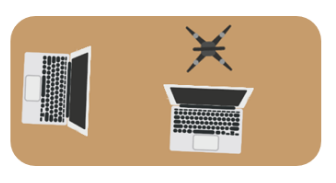
\includegraphics[scale=1.0]{Diagrams/Test_Setup.PNG}
   \caption{The Test Setup for the Iterative Usability Testing. Qualitative data were collected through audio and video recordings (represented by the tripod) of the stakeholders. The computer on the left side is used to take notes and record the initial observations during the tests. The post-survey test was also conducted in this computer. The computer on the right side is for the prototype system. When testing involves two stakeholders, they are positioned far from each other.}
    \label{fig:testsetup}
\end{figure}
\end{comment}
\subsection{Iterative Usability Testing}
We performed usability tests to determine the effectiveness of the prototype; whether it is a usable and collaborative timetabling application based on the usage of the key personnel involved. These were conducted in an environment wherein audio and visual disturbances were at a minimum. The participants were the stakeholders, the Academic Programming Officer (APO) and a Department Vice-Chair. Consent forms were provided before the respective tests. After they have given their consent, we oriented them with our goals and their tasks for the tests. They were also encouraged to follow a think-aloud protocol. This was done to allow the team to capture their thought process throughout the course pre-enrolment process. The stakeholders performed tasks depending on their actual roles namely:  course scheduling for the APO and faculty loading for the Vice-Chair. The were asked to do these roles using the latest ASSYSTX prototype. A total of three iterative testings were done spanning multiple versions of the prototype. 

The first iteration prototype focused on the gathering of feedback about the interface itself. This allowed the team to understand the visual preferences and the arrangement of elements in the prototype depending on the specific needs of the key personnel. This UT was tested using the task completion test. The first prototype was primarily designed to check if the system follows usability heuristics for good user interfaces. This iteration also inquired on how to improve the interaction design of the system. Some of the completed tasks are represented through a scoring system of 1 - 3: Accomplished being the highest score (3), Accomplished but with difficulty (2) representing the middle score, and Failed (1) as the lowest score. The tasks can be found in Table \ref{tab:tasks1}.
\begin{table}
  \centering
  \caption{Iteration 1 Tasks}~\label{tab:tasks1}
  \addtolength{\tabcolsep}{2pt} 
  \begin{tabular}{p{0.5cm}|p{6.5cm}}
  	\toprule
    \rule{0pt}{8pt}No. & Task \\[2pt]
    \toprule
    T1 & Find the place in the website where all the offerings are listed \\
    T2 & Modify a course offering \\
    T3 & Add a new course offering \\
    T4 & Know where to find how to send concerns and where to find received concerns \\
    \bottomrule
  \end{tabular}
  \addtolength{\tabcolsep}{-2pt} 
\end{table}
The second iteration of usability testing gave emphasis to the functionality of the timetabling features of the system. The testing done was not only to confirm if the system improved compared to the previous iteration, but also to validate its effectiveness with the intent of further improving the over-all interaction design. In this round of testing, the completion time it took to finish a task was recorded. The metric followed the same scoring convention as with the previous iteration. The tasks included in this round of testing contained more use-cases than the previous iteration. These are listed in Table \ref{tab:tasks2}. In order for us to further understand these results, we administered a post-test mixed-method interview  with the key personnel who participated in the said testing. This allowed us to further understand what the participant had experienced in using the system features. We can see in Table \ref{tab:scoring_scheme}, the results from the evaluation with answers ranging from the scale of 1 - 4, with 1 (Strongly Disagree) being the lowest, and 4 (Strongly Agree) being the highest. The questions for the survey can be found in Table \ref{tab:itr2_questions}. 

\begin{table}
  \centering
  \caption{Iteration 2 Tasks}~\label{tab:tasks2}
  \addtolength{\tabcolsep}{2pt} 
  \begin{tabular}{p{0.5cm}|p{6.5cm}}
  	\toprule
    \rule{0pt}{8pt}No. & Task \\[2pt]
    \toprule
    T1 & Modify course offering and check if changes made by another role are saved. \\
    T2 & Deload a Faculty \\
    T3 & Raise concerns and receive concerns from another role \\
    T4 & Track the changes made through revision history \\
    \bottomrule
  \end{tabular}
  \addtolength{\tabcolsep}{-2pt} 
\end{table}

\begin{table}
  \centering
  \caption{Post-Test Survey Scoring Scheme}~\label{tab:scoring_scheme}
  \addtolength{\tabcolsep}{2pt} 
  \begin{tabular}{p{1cm}|p{5cm}}
  	\toprule
    \rule{0pt}{8pt}Score & Definition\\[2pt]
    \toprule
    4 & Strongly Agree \\
    3 & Agree \\
    2 & Disagree \\
    1 & Strongly Disagree \\
    \bottomrule
  \end{tabular}
  \addtolength{\tabcolsep}{-2pt} 
\end{table}
The third iteration of testing focused on the discovering and measuring collaboration between the different users and key personnel. Both stakeholders were present in the same room and simultaneously used the  latest version of the prototype. However, verbal communication was discouraged. The test was designed to validate if multiple users can accomplish their tasks successfully and collaboratively while being able to communicate within the messaging feature of the system. The tasks of the participants for this iteration are listed in Table \ref{tab:tasks3}. For this specific test, a 0 - 4 scoring scheme was used. The corresponding definition of each score can be found in Table \ref{tab:itr3_scoring_scheme}. Similar to the previous iteration, a post-test survey was also administered. The questions are similar from the previous testing, as seen in Table \ref{tab:itr2_questions}, so that we can see if there are changes in the answers of the participants. 

\begin{table}
  \centering
  \caption{Iteration 3 Tasks}~\label{tab:tasks3}
  \addtolength{\tabcolsep}{2pt} 
  \begin{tabular}{p{0.5cm}|p{6.5cm}}
  	\toprule
    \rule{0pt}{8pt}No. & Task \\[2pt]
    \toprule
    T1 & Successfully create and modify a course across all users \\
    T2 & Check if changes made by a user reflects to the other user \\
    T3 & Raise concerns to the concerned user \\
    T4 & Track changes made by all users \\
    \bottomrule
  \end{tabular}
  \addtolength{\tabcolsep}{-2pt} 
\end{table}
\begin{table}
  \centering
  \caption{Iteration 3 Test Scoring Scheme}~\label{tab:itr3_scoring_scheme}
  \addtolength{\tabcolsep}{2pt} 
  \begin{tabular}{p{1cm}|p{5cm}}
  	\toprule
    \rule{0pt}{8pt}Score & Definition\\[2pt]
    \toprule
    4 & Accomplished Easily \\
    3 & Accomplished but with Confusion \\
    2 & Accomplished but Assisted \\
    1 & Accomplished by Mistake \\
    0 & Did not accomplish \\
    \bottomrule
  \end{tabular}
  \addtolength{\tabcolsep}{-2pt} 
\end{table}
\begin{table}
  \centering
  \caption{Criteria Used for Evaluating Collaboration}~\label{tab:itr2_questions}
  \addtolength{\tabcolsep}{2pt} 
  \begin{tabular}{p{.5cm}|p{2.75cm}|p{.5cm}|p{2.70cm}}
  	\toprule
    \rule{0pt}{8pt}No. & Task & No. & Task\\[2pt]
    \toprule
    Q1 & I am able to share my work with a person from a different role &  Q12 & I am able to track which person made what changes quickly\\
    Q2 &  I am able to see the work of a person from a different role  & Q13 & I am able to raise concerns to a person from a different role quickly\\
    Q3 & I am able to track which person made what changes & Q14 & I am able to receive concerns from a person from a different role quickly\\
    Q4 & I am able to raise concerns to a person from a different role & Q15 & I can collaborate with the other role through the system quickly\\
    Q5 & I am able to receive concerns from a person from a different role & Q16 & I am able to share my work with a person from a different role easily\\
    Q6 & I can collaborate with the other role through the system & Q17 & I am able to see the work of a person from a different role easily\\
    Q7 & I can easily see the contents of the system & Q18 & I am able to track which person made what changes easily\\
    Q8 & I can easily find what I'm looking for in the system & Q19 & I am able to raise concerns to a person from a different role easily\\
    Q9 & Everything I need to do my tasks are available  & Q20 & I am able to receive concerns from a person from a different role easily\\
    Q10 & I am able to share my work with a person from a different role quickly & Q21 & I can collaborate with the other role through the system easily\\
    Q11 & I am able to see the work of a person from a different role quickly & & \\
    \bottomrule
  \end{tabular}
  \addtolength{\tabcolsep}{-2pt} 
\end{table}
Feedback gathered were both qualitative and quantitative data in form. Insights came from interviews and audio-video recordings. The video recordings used includes a face camera to observe the facial expressions of the testers and the screen-capture of the system-interactions made by the testers during the test. Figure \ref{fig:cvc_testing} shows a screenshot of the face camera of the Vice Chair tester along with the screen-capture. Quantitative data was collected from the \textit{Task Completion Test Scores} and \textit{Post-Test Surveys} that the users were asked to answer after an iteration task test. 

% Insert here figures describing the UT setup
\begin{figure*}[]
\centering
   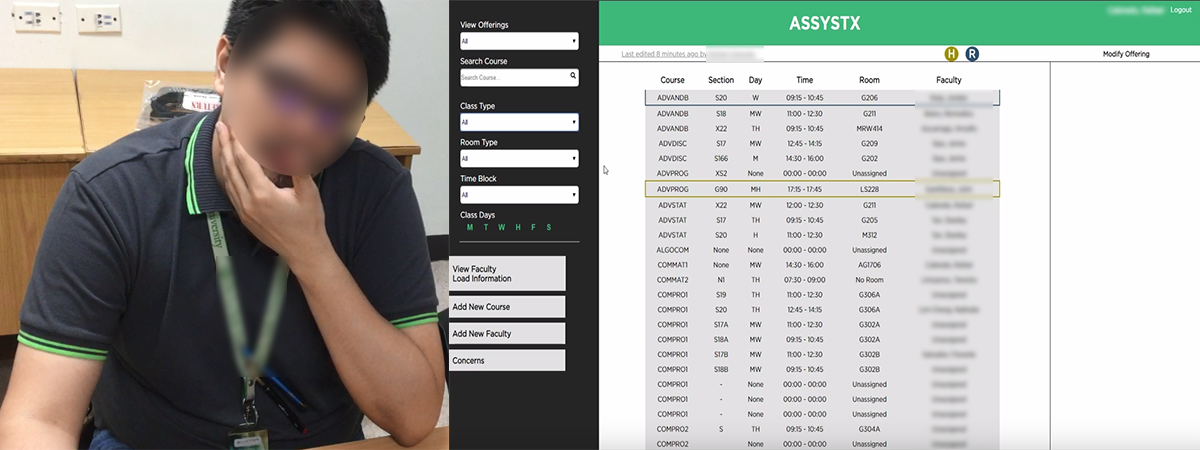
\includegraphics[scale=1.5,keepaspectratio]{PCSC2019_latex/Tests/sirTighe.png}
   \caption{Testing: The computer's face camera captures reactions of the participant while also capturing what he sees on the screen while using the system}
    \label{fig:cvc_testing}
\end{figure*}
% Guide questions, objectives discussions

\section{Results and Findings}
\subsection{System Design}
There are a total of six modules that were designed for ASSYSTX. The \textit{Shared Work Space Module} enables multiple users to use and share the system with a graphical user interface. The module is also responsible in creating the shared work space for the users to collaborate with when performing their respective tasks such as Faculty Loading and Course Scheduling. The \textit{Offerings Management Module} handles all features relating to the maintaining the different course offerings. The module handles creating a course offering; changing its status; assigning a time slot, room, and faculty; and dissolving an offering. Conflict resolution and rule violation checking when assigning a room or faculty are also implemented within this module. Similar to the \textit{Offerings Management Module}, the \textit{Profiles Management Module} handles all features for course and faculty profiles. These profiles are used for creating a course offering. Thus, this module is responsible for the creation and management of courses and faculty. Faculty deloading is also performed under this module. The \textit{Concerns Management Module}, meanwhile, is responsible for raising and receiving concerns. This module ensures that the concerns reach the target receiver. Acknowledgement and notifications for messages are received by the target user. The \textit{Work Space History Module} is in-charge of auditing the changes made in the course offerings list of the system. These logs are then relayed to the \textit{User Interface Module} for display in the work space. Lastly, the \textit{User Activity Module} tracks the user actions within the system. The module records the course offering currently being modified, the user's last seen concern and change log. These are used for notifications and help in inciting collaboration within the work space.
\begin{figure}[h]
   \centering
   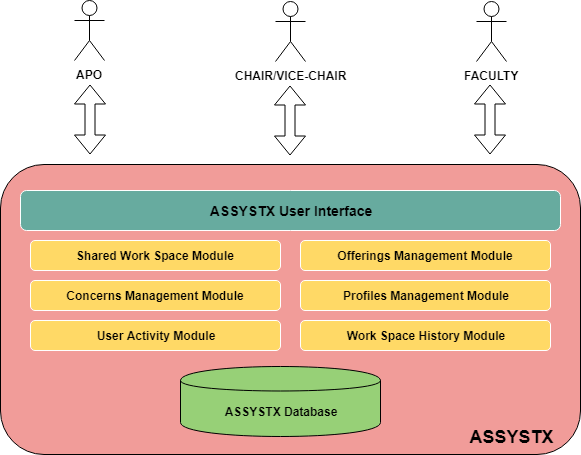
\includegraphics[scale=0.4]{Diagrams/System_Architecture.png}
   \caption{ASSYSTX System Architecture. The ``Shared Work Space" module allows users to collaborate through the interface to access the other modules such as ``Concerns Management" and ``Work Space History" modules to create a course schedule}
    \label{fig:pipelinediagram}
\end{figure}
\begin{figure*}[h]
   \centering
 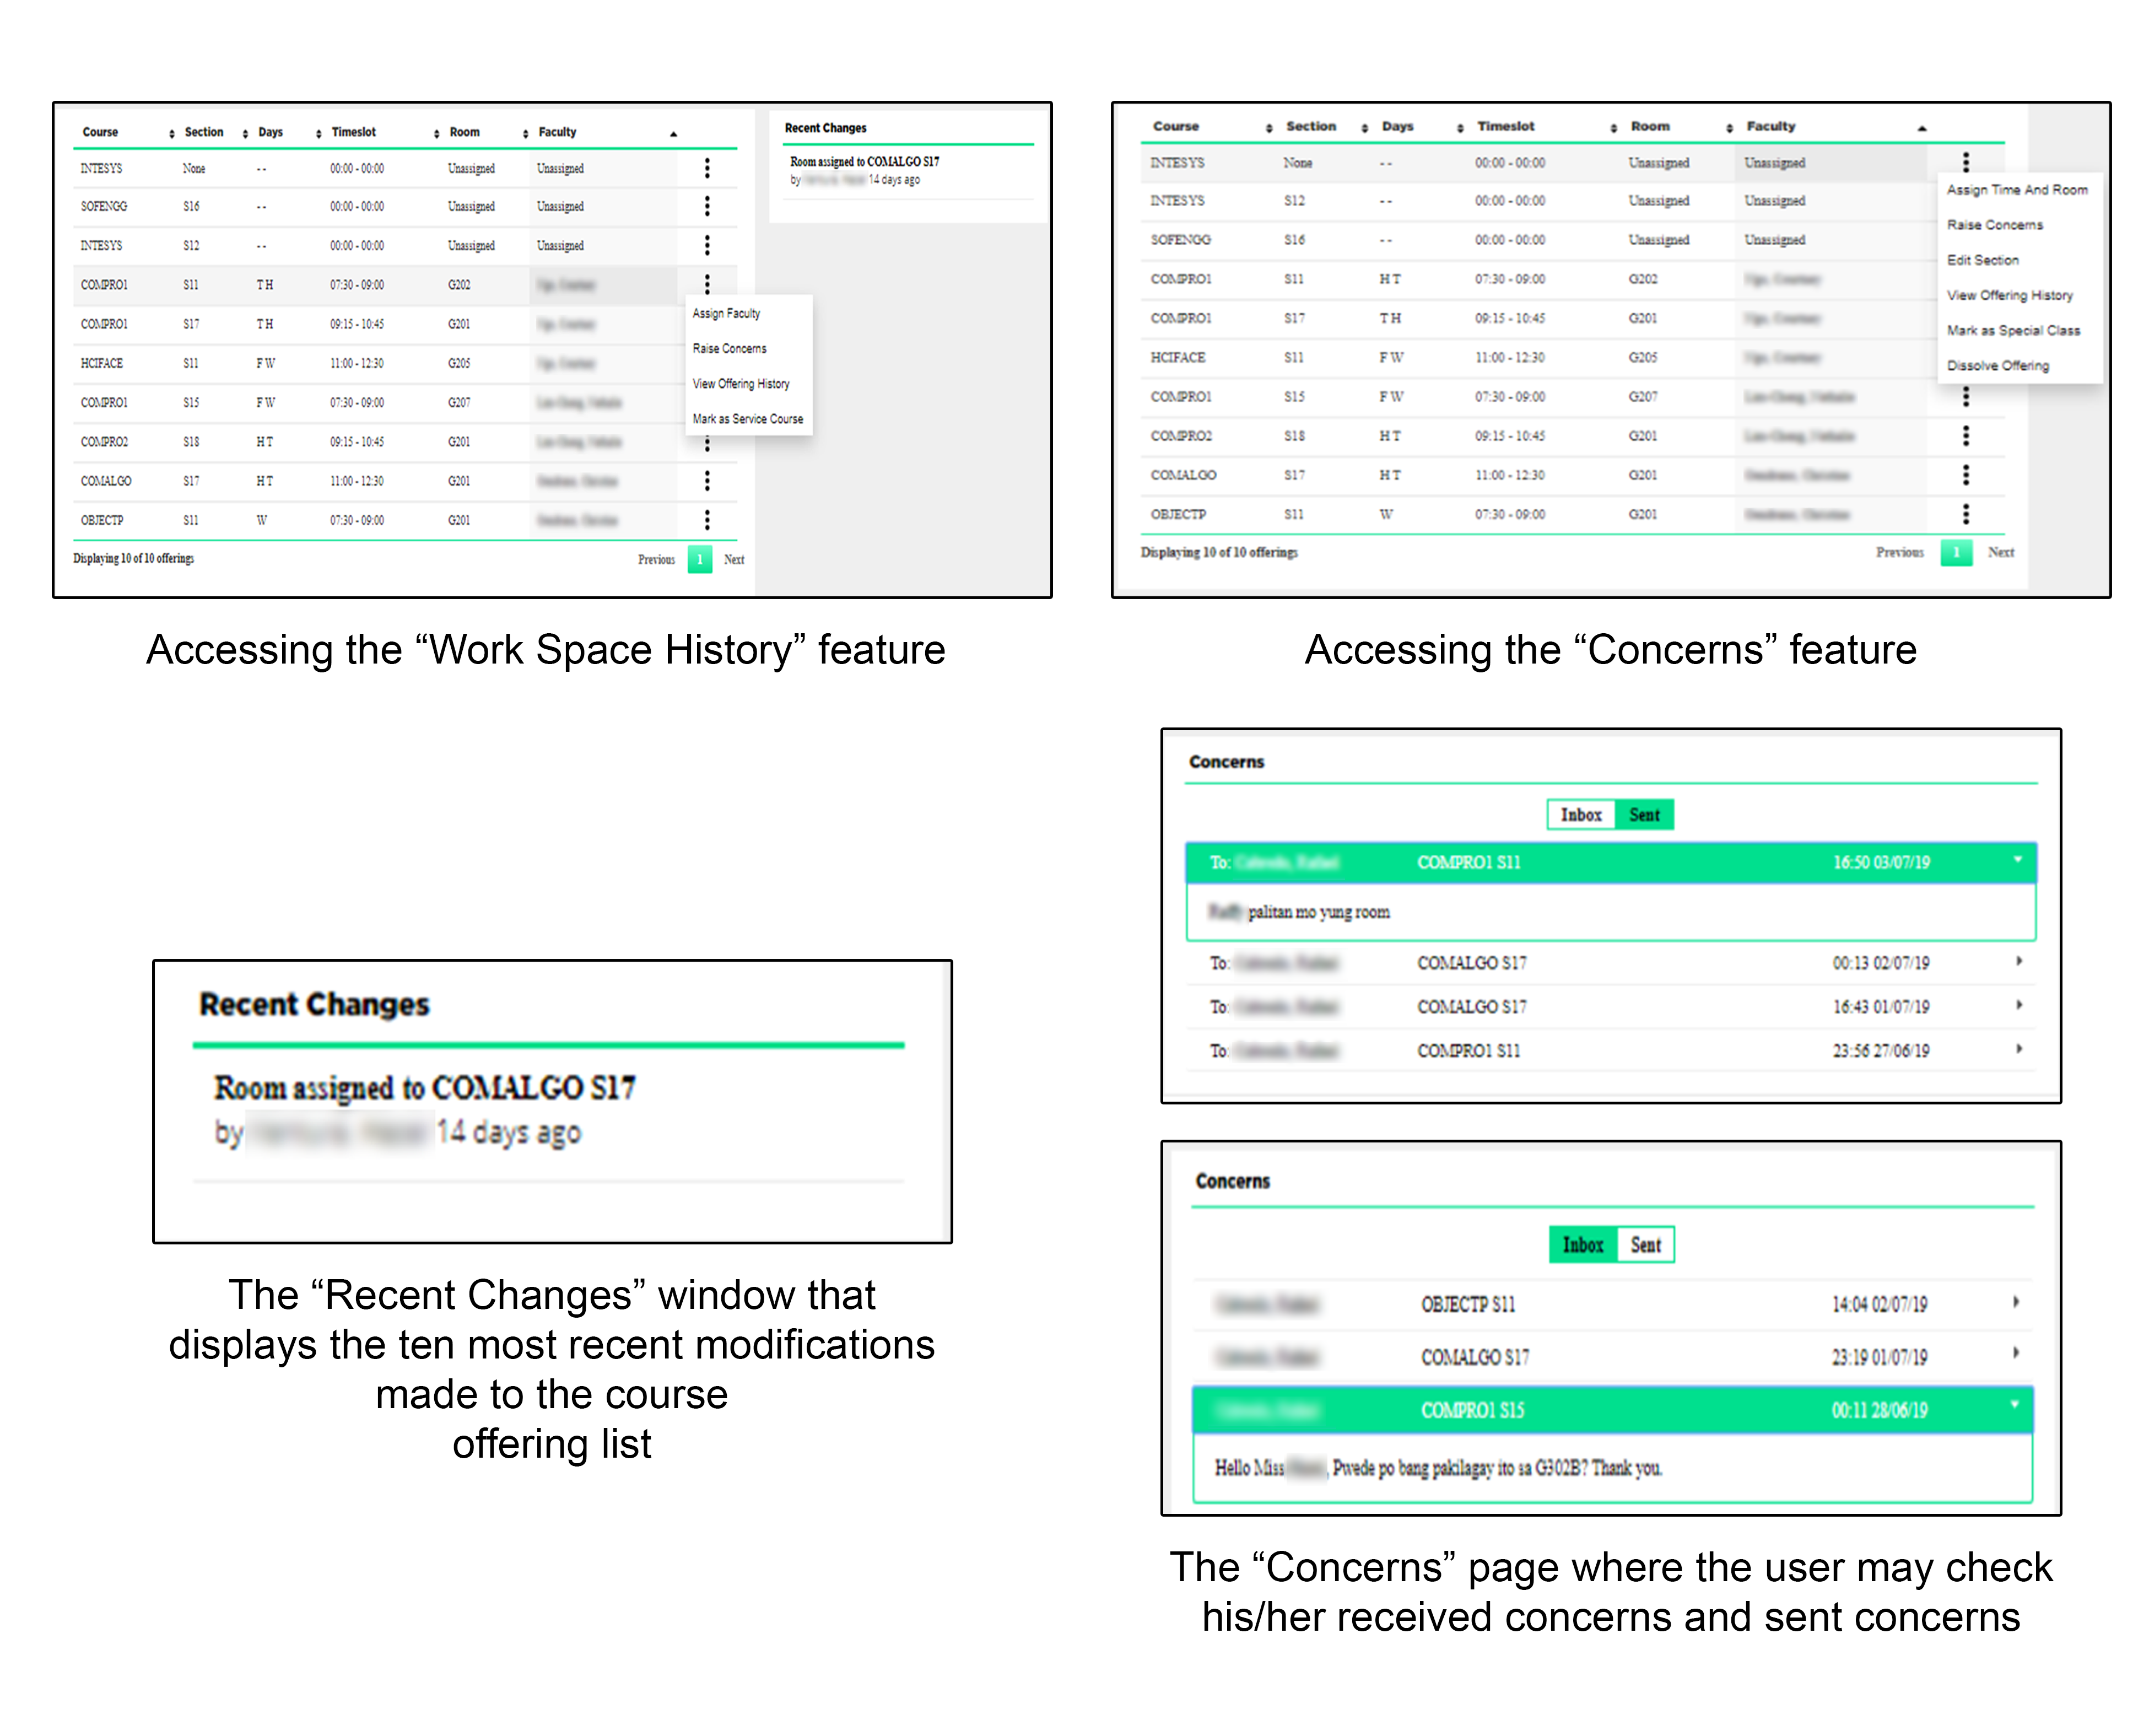
\includegraphics[width=\textwidth,height=\textheight,keepaspectratio]{PCSC2019_latex/Screenshots/assystxScreenshots.png}
   \caption{Two of the ASSYSTX Collaborative Features: Work Space History and Concerns} \label{fig:assystxScreenshot}
\end{figure*}
\subsection{Usability Tests}
% Insert here UT results (table)

% Insert here table comparing the UT scores
During every iteration, we did a mixed method evaluation of the system. Quantitative scores were collected and collated into a summary of scores, arranged per cluster. These can be found at Table \ref{tab:summarized_post_test_cluster}. It can be observed from the table that the average rating per cluster improves as the iterations go on. This can imply that there are improvements in the user experience of the system. With the \textit{Collaborative Features} cluster having improved the most, followed by the \textit{Speed} cluster, \textit{Ease of Use}, and finally \textit{Accessibility}. The increase in the \textit{Collaborative Features} cluster may be attributed to the fact that the improvements on the collaborative features, especially the raising of concerns, which allows users to communicate , negotiate, and plan out what is needed next for the schedule. Compared to the previous iteration, the participants were able to easily utilize the concerns feature. Improvements in the Work Space History, which allows users to check on the progress made by other users to guide them in their next courses of action can also be credited for the increase.  In order to validate whether the rise in scores were significant enough for each cluster, We performed hypothesis testing between the two iterations' scores. The following null and alternative hypotheses are: 
 \label{list:significance_testing}
 \begin{itemize}
    \item $H_0$ - There is no significant difference between the mean scores of Iteration 2 and 3 per cluster.
    \item $H_\alpha$ - There is a significant difference between the mean scores of Iteration 2 and 3 per cluster.
\end{itemize}
The sample size was identified through t-statistic, or total number of questions, are less than 30. Lastly, the significance value will be 5\% or 0.05. If the computed p-value is less than 0.05, then the null hypothesis can be confidently rejected and accept the alternative hypothesis. The results of the hypothesis testing can be seen at Table \ref{tab:summarized_significance_testing}.

Three clusters, Collaborative Features, Speed, and Ease of Use, had a p-value of less than 0.05, indicating a significant difference in the scores. While the scores of the Accessibility cluster itself had improved, it remains to be the lowest-scored cluster and not having much significant difference. This may be due to lack of prompts and call to action to guide the user in the system. The unfamiliarity of the participant to system may also be attributed to this.
\begin{table}
\centering
\caption{\label{tab:summarized_post_test_cluster}Summarized Post-Test Survey Cluster Scores from Iteration 2 - 3}
\begin{tabular}{|l|l|l|l|l|l|l|}
\hline
\textbf{Cluster} & \textbf{I2} & \textbf{I3} & \mu & \textbf{I3 - I2} \\\hline
Collaborative Features & 3.00 & 3.75 & 3.40 & 0.75\\\hline
Accessibility & 2.67 & 3.00 & 2.80 & 0.33\\\hline
Speed & 3.00 & 3.58 & 3.30 & 0.58\\\hline
Ease of Use & 3.00 & 3.67 & 3.30 & 0.67\\\hline
Average &  &  &  & 0.58\\\hline
\end{tabular}
\end{table}
\begin{table*}
\centering
\caption{\label{tab:summarized_significance_testing}Summarized Significance Testing Results}
\resizebox{15cm}{!}{\begin{tabular}{|l|l|l|l|l|l|l|}
\hline
\textbf{Cluster} & \textbf{I2 Mean} & \textbf{I2 St.Dev.} & \textbf{I3 Mean} & \textbf{I3 St.Dev} & \textbf{t-statistic} & \textbf{p-value}  \\\hline
C1. Collaborative Features   & 3.000 & 0.000  & 3.750 & 0.250 & 7.348 & 0.000  \\\hline
C2. Accessibility            & 2.667 & 0.471  & 3.000 & 0.000 & 1.225 & 0.374 \\\hline
C3. Speed                    & 3.000 & 0.000  & 3.580 & 0.344 & 4.159 & 0.004 \\\hline
C4. Ease of Use              & 3.000 & 0.000  & 3.667 & 0.236 & 6.928 & 0.000 \\\hline
\end{tabular}}
\end{table*}
\begin{figure}[h]
   \centering
   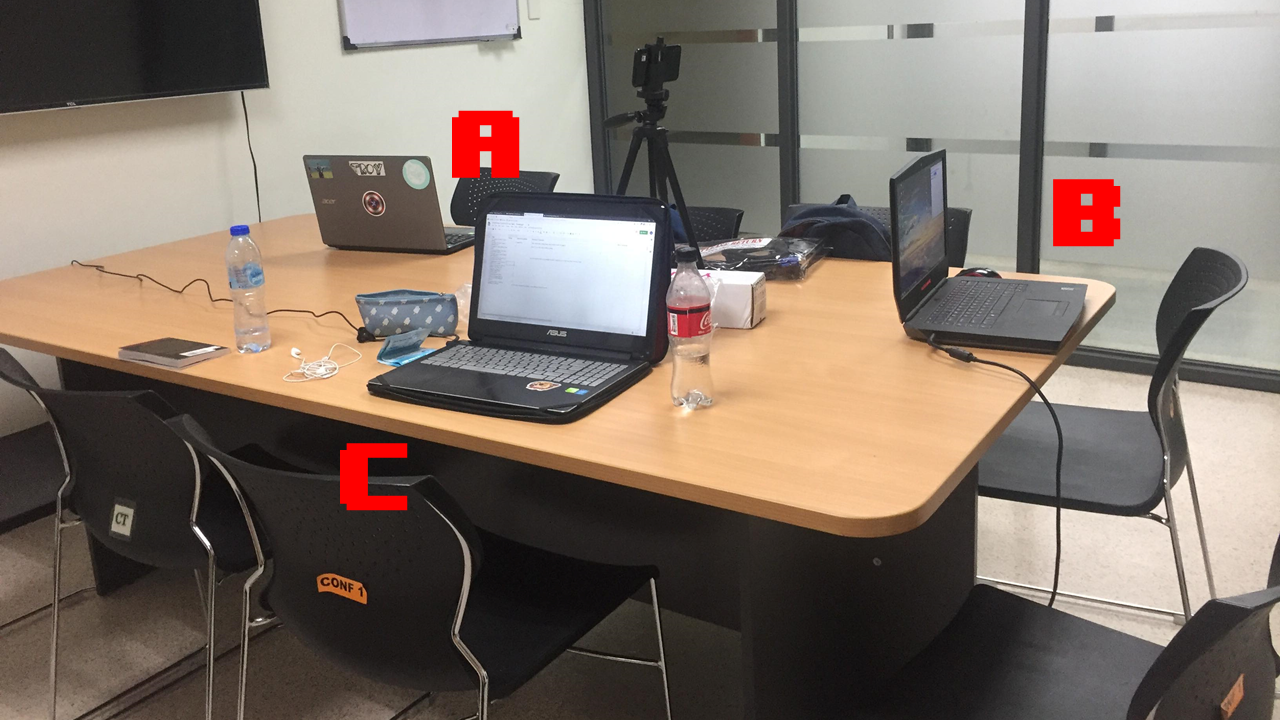
\includegraphics[scale=0.2]{PCSC2019_latex/Tests/test_setup_iteration3.png}
   \caption{Iteration 3 Test Setup: The participants are placed in a room with minimal noise and distractions. The Vice-Chair is seated in Computer A, the APO in Computer B, while the datalogger is in Computer C.}
    \label{fig:itr3_testsetup}
\end{figure}
\subsection{Human-Human Collaboration Factors}
We were able to observe some collaboration factors that involved two key personnel roles interacting with each other. In one given scenario, stakeholders must work together to create an agreeable schedule for a given term, taking into account variables that are present for that specific trimester. The APO preempts the process through creating a list of course offerings based on the college's flowcharts and batch size. We were able to observe that the APO then proceeds to assign a room and time slot for the course offerings. The APO may be able to create more offerings following a request from the Chairs/Vice-Chairs. This is made easy by the communication and notification modules of ASSYSTX. The Chairs/Vice-Chairs, meanwhile, are in-charge of assigning faculty to the course offerings. Criteria for assigning faculty include past teaching experiences with a certain course, his/her areas of expertise, and his/her current work load. Because of the Raise Concern module, concerned faculty may send their request to the APO about assigning specific time slots on specific offerings to ascribe to their planned faculty assignment. This may or may not be followed by the APO. 
% ^ look at what I did here. you could do it to the next ones

%(no need to rewrite troy. sisingitan niyo lang ng words... look what ill do here...
In the last iteration, the college APO and the Software Technology Vice-Chair were asked to test the system. New features and modules were introduced like Recent Changes and Live Editing to further facilitate collaboration. The test setup can be seen in Figure \ref{fig:itr3_testsetup}, wherein the Vice-Chair was seated in position `A', the APO in `B', and a designated datalogger in `C' that would observe the progress and reactions of both parties. For this task, the APO is to create a course offering and had assigned a room to it. The Chair is made aware that the APO is assigning rooms and knows exactly what are they specifically working on. This is made possible by the Live Editing feature in the Shared Workspace. Knowing the APO is done with these courses, the Vice-Chair can then assign a faculty member to that course. Following an update in the Recent Changes window, the APO attached a concern to a course offering which the Vice-Chair acknowledged.

%we need to insert how we "force" them to collaborate using our features 

%look at what I did here 
%>> The Chair is made aware that the APO is assigning rooms and knows exactly what are they specifically working on. This is made possible by the Live Editing feature in the Shared Workspace. Knowing the APO is done with


\textit{Human-Human Collaboration} allows multiple stakeholders to contribute and coordinate in handling the factors in creating the schedule. The APO who is responsible for providing the courses needed to be offered in the term will need to coordinate with the Chairs responsible for loading the faculty inside those courses. In assigning the faculty of a given course, there might be a need to change its properties (e.g. time slot, room assigned) in order for it to conform to his/her needs.


\subsection{Human-Computer Collaboration Factors}
The ASSYSTX system acted as the collaboration tool for the CCS timetabling process. In the last iteration, it acted as the medium where the APO and Vice-Chair testers simulated the timetabling process. When the APO had created a new course offering, the Vice-Chair was easily able to find it through the Shared Workspace, which enabled him to assign a faculty to the course with ease. Similarly, the APO was able to verify that the Vice-Chair had assigned a faculty to the course offering she created with the Recent Changes feature. When the APO had attached a concern to another course offering, the Vice-Chair was immediately notified and was able to acknowledge the concern. 

The system provided an avenue where users can perform the basic timetabling tasks such as creating course offerings and modifying an existing course offering along with facilitating the collaboration between users. The Shared Workspace regularly updates the course offerings and concerns so that the users can finish faster with their pending tasks. The Offering History and Recent Changes features keeps track of changes made in the course offerings by the users so they can make plans on their next course of action.

In \textit{Human-Computer Collaboration} there is a clear division of work between the user and the system. In the context of timetabling, the actual manipulation of courses and faculty are handled by the users, while the system only assists through features like notifications, messaging, and revision history. It also allows for multiple users to synchronously work on the course schedule without conflicts with the Shared Workspace. The system also has a rule-checker module that determines whether the schedule conforms to rules that are set by the college (e.g. faculty teaching loads, time-slot conflicts).  

\section{Conclusion and Future Work}
In this study, we were able to observe and understand how key personnel from a specific university collaborate during enrollment. These findings are seen in Section 4.4. We were able to derive and formulate features on how to design ASSYSTX which can be see in Section 4.1.  Through usability tests we were able to observe how these design implications affect collaborative activities as seen in Section 4.2. From our post-test survey scores, the Collaborative Features garnered the highest mean score with 3.40 (out of 4.00), highlighting their positive effect towards better collaboration. Lastly, we were able to reflect on these collaborative activities as seen in the Results and Findings section.

%We were able to iteratively develop a collaborative timetabling application through ASSYSTX. Feedback after tasks was the general weakness of the system, as it hampered the accessibility of the system, both qualitatively and quantitatively. The collaborative features received the highest average score, albeit based off one test. All the tasks were accomplished by both participants and were done collaboratively in the third iteration. The participants did not deviate from the actual timetabling process (e.g. APO creates offering and assigns time and room before Vice-Chair assigns faculty) in all three iterations. The third iteration version of the system does allow both participants to modify the same course offering, however this was not explored nor considered.

For future work, we intend to do more of testing the system with conflict-driven scenarios that require collaboration. The tests we performed only concerned with the collaborative features' functionality and how they help the user complete a task. We intend to measure its thorough effectiveness from these given scenarios. The authors also believe there is a need to perform tests with more than two participants. A speed metric for comparison between performing tasks with and without the collaborative features can also be considered to evaluate the system's responsiveness. 



\bibliographystyle{ACM-Reference-Format}
\bibliography{references}

\end{document}
